\documentclass{article}
\usepackage[utf8]{inputenc}
\usepackage{graphicx}

\title{Lab 6 Redes: "Sockets"}
\author{Vicente Lopez\\Esteban León\\Sebastian Antón\\Jorge Ramirez\\Profesor: Jose Alejandro Perez\\Ayudante: Alexis Inzunza}
\date{Junio 2017}

\usepackage{natbib}
\usepackage{graphicx}

\begin{document}
\begin{figure}[h]

\includegraphics[width=0.45\textwidth]{logo_udp.png}
\maketitle
\end{figure}

\section{Indice}

2 Introducción -------------------------------------------------2\\
3 Desarrollo del experimento-------------------------------2\\
4 Analisis y preguntas----------------------------------------3\\
5 Conclusión -------------------------------------------------- 4\\
6 Bibliografia -------------------------------------------------- 5\\\\\\\\\\\\\\\\\\\\\\\\\\\\

\section{Introducción:}

Para esta experiencia creamos dos programas en python correspondientes a un cliente y un servidor que establecen comunicación mediante el tipo de dato “socket” que permite la comunicación entre un cliente y un servidor, los cuales tienen el protocolo de transporte TCP.\\\\

\section{Desarrollo del experimento:}

En esta actividad programaremos dos programas, uno correspondiente al cliente y otro a un servidor. Dichos programas, con la ayuda del tipo de dato “socket”, se comunican entre sí mediante los métodos que contiene este tipo de dato.
Adicional a la comunicación que debe mantener el cliente con el servidor, es necesario que el servidor mantenga comunicación con más de un cliente y para ello hicimos uso de la librería “threading”, la cual nos permite tener distintos procesos corriendo de manera paralela a otros procesos.
\\
Ademas analizamos el trafico de datos por wireshark los cuales han sido enviados desde un pc a el servidor, como por ejemplo, como el paquete TCP del pc con ip 172.16.32.105 llego al pc destino con ip 172.16.32.104\\\\

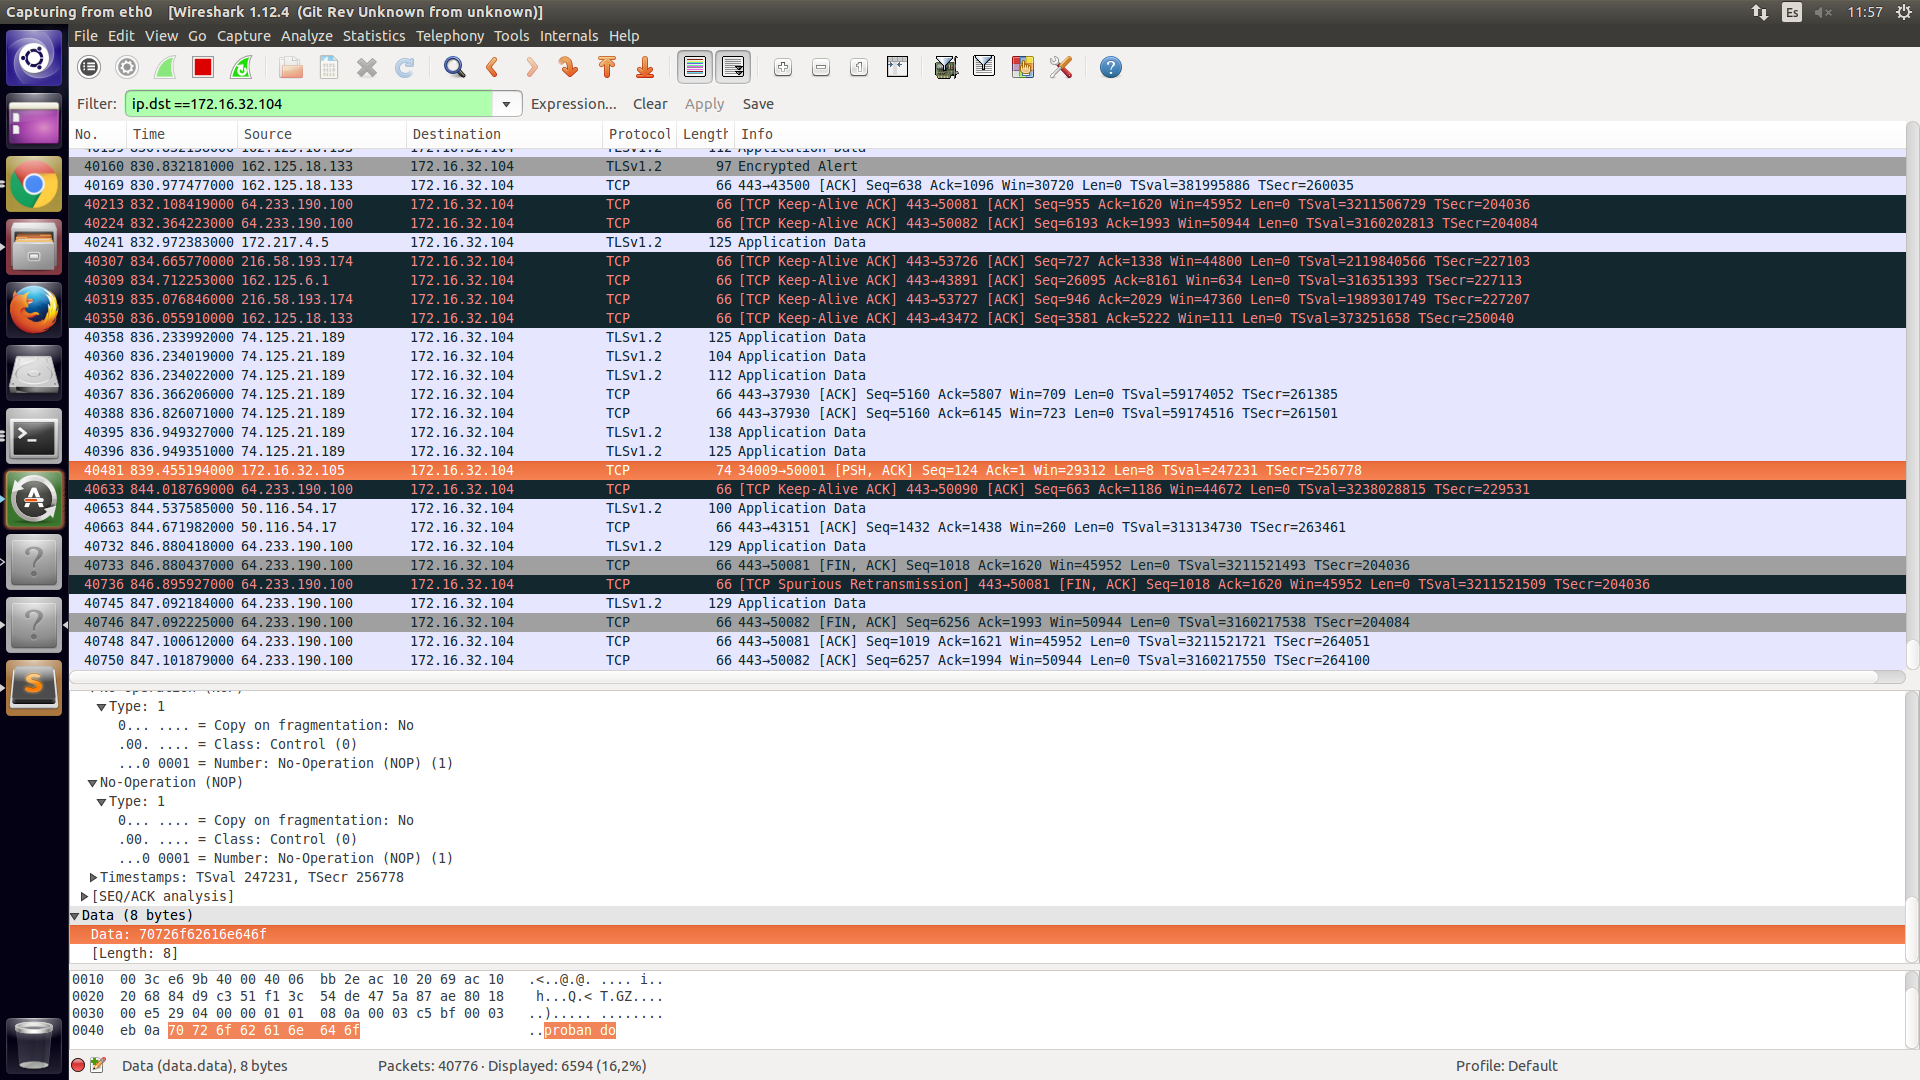
\includegraphics[width=1\textwidth]{Wire.png}\\\\
-*El paquete esta marcado con naranjo\\\\

\subsection{Análisis y preguntas:}

1.- explique el funcionamiento del envío y recepción de información para su algoritmo, respondiendo a las interrogantes ¿Qué se envía? ¿Cómo se envía?\\\\

Primero se arma el servidor y se prepara para poder recibir el mensaje, luego de que esta en modo espera el servidor en el codigo "sock, addr =s.accept()", el cliente arma un paquete TCP para ser enviado posteriormente en el codigo "c.send(i)" por una direccion y un puerto, luego de enviar el paquete, el servidor que estaba en modo espera, lo recibe y entra en el codigo "t=threading.Thread(target = Msn,args=(sock,addr))" para hacer un proceso mientras el servidor espera la llegada de otro cliente.\\\\

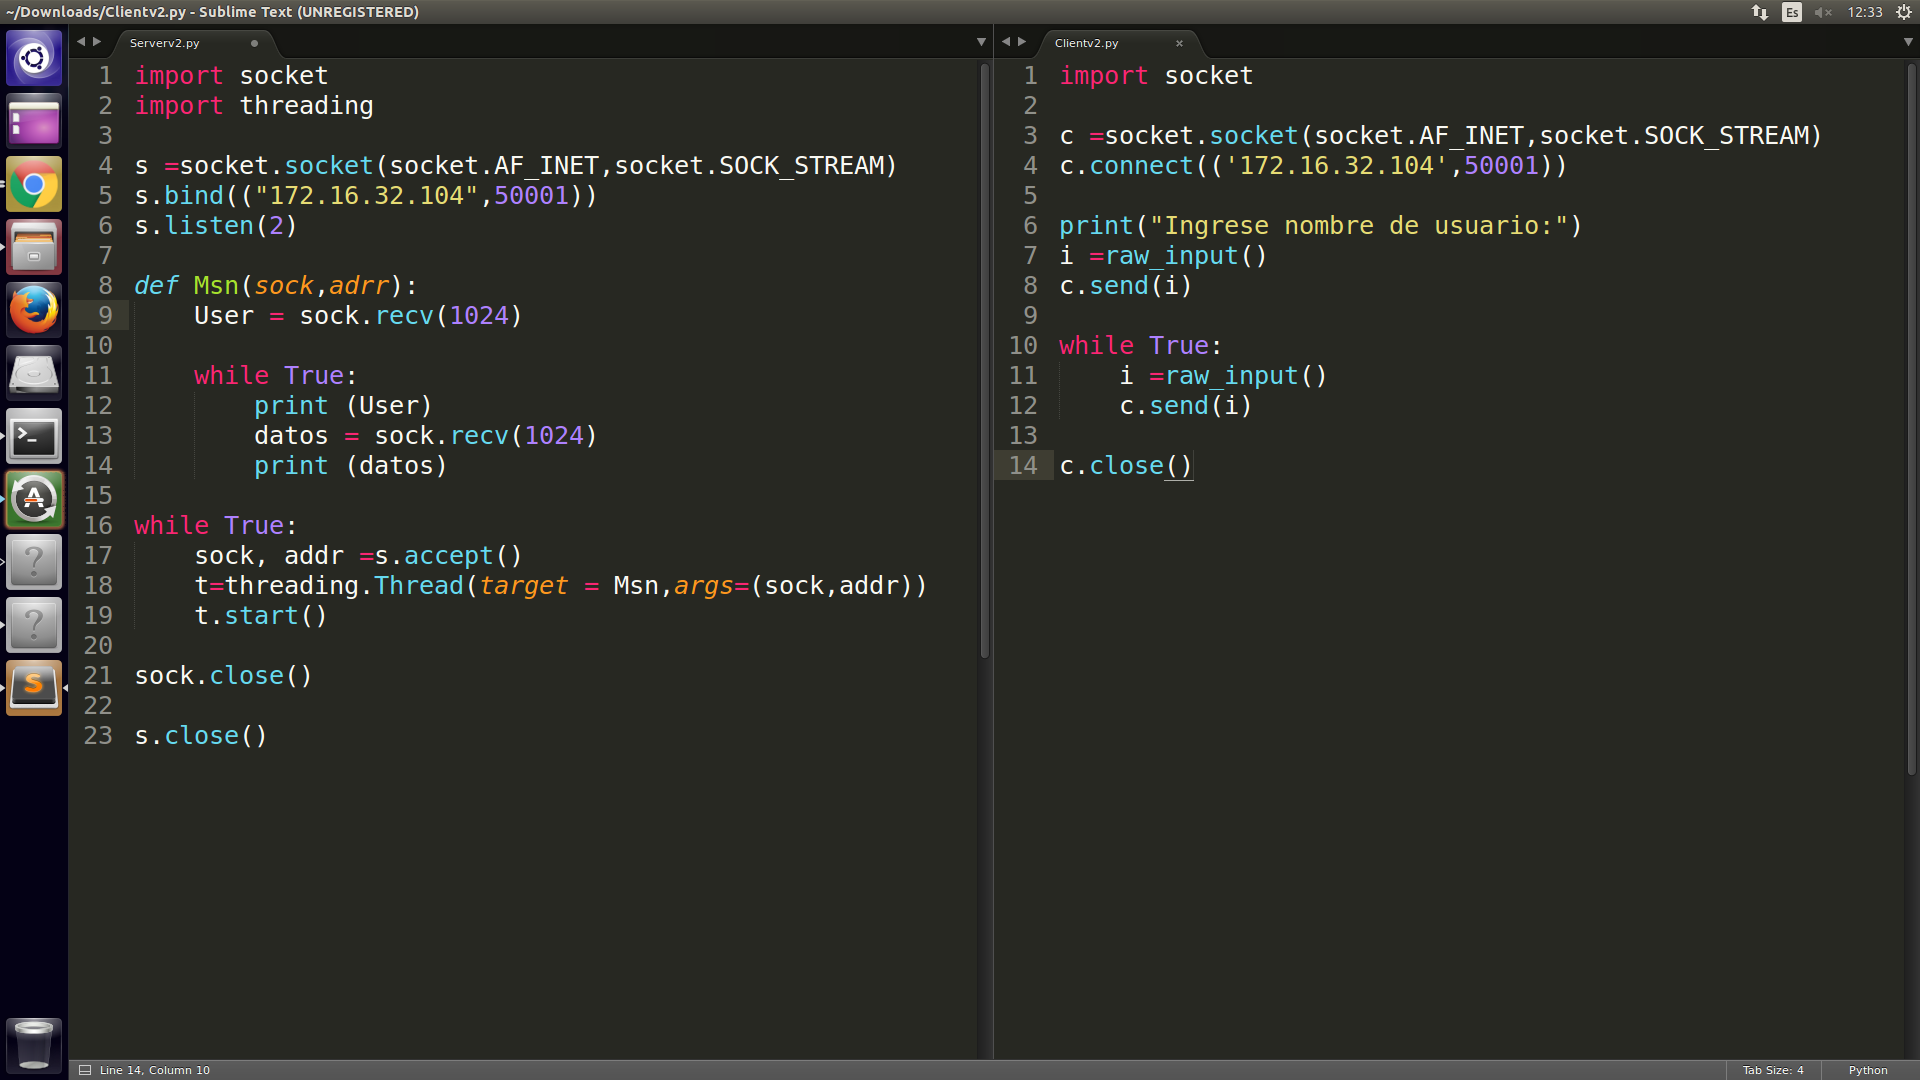
\includegraphics[width=1\textwidth]{clientserver.png}\\\\

2.- ¿Por qué el puerto que muestra el servidor al generar la conexión no es el mismo que el escrito en el algoritmo del cliente?\\\\

Esto ocurre debido a que se genera un redireccionamiento de puertos debido a que se trata de ingresar a un computador en concreto con una ip privada adentro de una lan privada. Las maquinas con Linux (como es en este caso) consiguen esto añadiendo reglas de iptables a la tabla nat.\\

3.- Si usted tuviese que realizar un videojuego con soporte multijugador utilizando sockets ¿Qué protocolo utilizaría? ¿Por qué?.\\

El protocolo UDP es un protocolo no orientado a la conexión, ya que se enfoca más en la comunicación unidireccional. La transferencia realizada por este protocolo, no corrobora si los datos fueron recibidos por el host destinatario y la conexión termina cuando se deja de enviar datos. Al contrario del protocolo TCP, que es destinado a la conexión, ya que cuando se envía un paquete con este protocolo, el host receptor comunica al emisor que los datos fueron entregados con éxito y de no ser así, solicita al emisor que el o los paquetes se envíen nuevamente, y la conexión se mantiene desde que inicia el envío hasta que se decide terminar con la conexión. Debido a lo anterior, es más apropiado utilizar el protocolo UDP, si bien no asegura si los datos fueron recibidos, en un videojuego con soporte multijugador, es necesario que todos los personajes se muevan al mismo tiempo, gracias a su velocidad (a diferencia del protocolo TCP que demora el doble de tiempo en enviar los datos y en esperar la respuesta de la recepción exitosa), el protocolo UDP es el ideal para lograr que todos los personajes puedan interactuar sin demoras.\\\\

4.- ¿Se puede utilizar cualquier número de puerto para cualquier aplicación? Explique..\\\\

No se puede ocupar cualquier numero de puerto, ya que desde el 1024 hacia abajo (sin incluirlo), son reservados del sistema operativo y usados por los protocolos HTTP (servidor Web), POP3/SMTP (servidor de e-mail), por ejemplo. Y para hacer uso de estos, es necesario contar con los permisos del administrador. En el caso de los puertos entre 1024 y 49151, si pueden ser usados para cualquier aplicación. 
Para los puertos entre 49152 y 65535, son llamados “dinámicos” y se asignan normalmente a las aplicaciones de clientes al iniciar conexiones del tipo Peer to Peer. 
Debido a esto, se sugiere utilizar puertos entre 1024 y 49151 para cualquier aplicación.\\\\

\section{Conclusión}

En esta experiencia comprendimos la importancia del protocolo TCP y sus diferencias con el protocolo UDP, conociendo sus beneficios y desventajas. Ahora somos capaces de elegir el protocolo adecuado según nuestra necesidad. 
Adicional a esto, fuimos capaces de comprender la comunicación que existe entre un servidor y un cliente mediante la librería “socket” y la comunicación entre dos o más clientes con el servidor de manera paralela, mediante la librería “threading”.\\

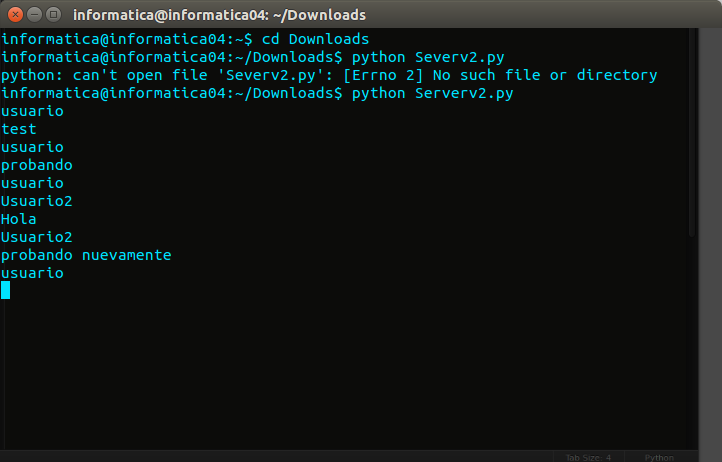
\includegraphics[width=1\textwidth]{server.png}\
*demostracion del servidor con 2 clientes simultaneos*\\\\\

\section{Bibliografia}
http://blogs.shephertz.com/es/2013/01/28/picking-the-right-communication-protocol-for-your-game/\\
http://www.marcelopedra.com.ar/blog/2009/08/09/tabla-de-puertos-tcp/\\
http://www.moraldonet.com.ar/info/reference/ports.htm\\

\end{document}